% Options for packages loaded elsewhere
\PassOptionsToPackage{unicode}{hyperref}
\PassOptionsToPackage{hyphens}{url}
%
\documentclass[
  a4paper,
]{article}

\usepackage{etoolbox}
% \setmainfont{Linux Libertine O}
\AtBeginEnvironment{quote}{\it\small}

\usepackage[toc,page,header]{appendix}
% \renewcommand{\appendixpagename}{\centering Appendices111}

% \usepackage[colorlinks=true, linkcolor=blue, urlcolor=blue, citecolor=blue, anchorcolor=blue]{hyperref}

\usepackage[]{mathpazo}
\usepackage{setspace}
% \usepackage{lmodern,bm}
% \usepackage{unicode-math}
\usepackage{amssymb}
\usepackage{amsmath}
% \usepackage{amsfonts}
\usepackage{ifxetex,ifluatex}
\ifnum 0\ifxetex 1\fi\ifluatex 1\fi=0 % if pdftex
  \usepackage[T1]{fontenc}
  \usepackage[utf8]{inputenc}
  % \usepackage{textcomp} % provide euro and other symbols
  % \usepackage{newtxtext,newtxmath}
  % \usepackage{mathptmx} \usepackage{tgtermes}
  % \usepackage{FiraSans} 
  % \usepackage[sfdefault]{FiraSans} \usepackage{FiraMono} \renewcommand*\familydefault{\sfdefault}
  % \usepackage{tgpagella}
  % \usepackage[utopia]{mathdesign}
  % \usepackage[math]{iwona}
  % \usepackage[sfdefault,scaled=.85]{FiraSans} \usepackage{newtxsf}
  % \usepackage{cmbright}
  % \usepackage{ccfonts,eulervm}  \usepackage[T1]{fontenc}
  % \usepackage[math]{kurier}
  % \usepackage{fourier}
  % \usepackage{mathpazo}
  % \usepackage{isomath}
  \else % if luatex or xetex
  % \usepackage{fourier}
  % \usepackage{mathpazo}
  % \usepackage{cmbright}
  % \usepackage{isomath}
  \usepackage{fontspec}
  \usepackage{unicode-math}
  \defaultfontfeatures{Scale=MatchLowercase}
  \defaultfontfeatures[\rmfamily]{Ligatures=TeX,Scale=1}
  % \setmainfont{Optima}
  % \setsansfont{Optima}
  % \usepackage{unicode-math}
  % \setmathfont{Optima}
  % \setmathfont{XITS Math}
\fi
% Use upquote if available, for straight quotes in verbatim environments
\IfFileExists{upquote.sty}{\usepackage{upquote}}{}
\IfFileExists{microtype.sty}{% use microtype if available
  \usepackage[]{microtype}
  \UseMicrotypeSet[protrusion]{basicmath} % disable protrusion for tt fonts
}{}
\makeatletter
\@ifundefined{KOMAClassName}{% if non-KOMA class
  \IfFileExists{parskip.sty}{%
    \usepackage{parskip}
  }{% else
    \setlength{\parindent}{0pt}
    \setlength{\parskip}{6pt plus 2pt minus 1pt}}
}{% if KOMA class
  \KOMAoptions{parskip=half}}
\makeatother
\usepackage{xcolor}
\IfFileExists{xurl.sty}{\usepackage{xurl}}{} % add URL line breaks if available
\IfFileExists{bookmark.sty}{\usepackage{bookmark}}{\usepackage{hyperref}}
\hypersetup{
  pdfauthor={Stone Fang (Student ID: 19049045)},
  hidelinks,
  pdfcreator={LaTeX via pandoc}}
\urlstyle{same} % disable monospaced font for URLs
\usepackage[margin=25mm]{geometry}
\usepackage{graphicx,grffile}
\makeatletter
\def\maxwidth{\ifdim\Gin@nat@width>\linewidth\linewidth\else\Gin@nat@width\fi}
\def\maxheight{\ifdim\Gin@nat@height>\textheight\textheight\else\Gin@nat@height\fi}
\makeatother
% Scale images if necessary, so that they will not overflow the page
% margins by default, and it is still possible to overwrite the defaults
% using explicit options in \includegraphics[width, height, ...]{}
\setkeys{Gin}{width=\maxwidth,height=\maxheight,keepaspectratio}
% Set default figure placement to htbp
\makeatletter
\def\fps@figure{htbp}
\makeatother
\setlength{\emergencystretch}{3em} % prevent overfull lines
\providecommand{\tightlist}{%
  \setlength{\itemsep}{0pt}\setlength{\parskip}{0pt}}
\setcounter{secnumdepth}{5}
\pagestyle{empty}

% \usepackage{ifthen}
% Using fancy headers and footers
\usepackage{fancyhdr}
\pagestyle{fancy}
\fancyhead{} % clear all header fields
\fancyhead[L]{COMP810 Data Warehousing and Big Data Assessment 2}
% \fancyhead[CO,CE]{\ifthenelse{\value{page}=1}{first page}
% {COMP810 Data Warehousing and Big Data Assessment 2}}
\fancyfoot{} % clear all footer fields
\fancyfoot[LO,RE]{Stone Fang (19049045)}
\fancyfoot[LE,RO]{\thepage}
\renewcommand{\headrulewidth}{0.4pt}
\renewcommand{\footrulewidth}{0.4pt}

\renewcommand*{\thefootnote}{ [\arabic{footnote}]}

\fancypagestyle{plain}{\pagestyle{fancy}}
\usepackage[noabbrev]{cleveref}
    \usepackage{tcolorbox}

    \newcommand{\sqloutputbegin}[1][SQL Output]{
        \hspace{0.5cm}
        \begin{minipage}[c]{0.93\linewidth} 
        \centering
        \begin{tcolorbox}[colback=gray!8, colframe=white,
            boxrule=0pt, coltitle=black,
            colbacktitle=gray!15, title={#1}]
        \centering
        \small}
    \newcommand{\sqloutputend}{
        \end{tcolorbox} 
        \end{minipage}}
\renewcommand{\labelenumii}{\theenumii}
\renewcommand{\theenumii}{\theenumi.\arabic{enumii}.}
\usepackage[style=alphabetic,backend=bibtex]{biblatex}
% redefine the booktitle macro or apacase directive to preserve the source casing for the booktitle field in the @inproceedings
\renewbibmacro*{booktitle}{\printfield{booktitle}}
% \DeclareFieldFormat{apacase}{%
%   \ifboolexpr{ test {\ifentrytype{inproceedings}}
%     and ( test {\ifcurrentfield{booktitle}}
%           or test {\ifcurrentfield{booksubtitle}} ) }
%     {#1}{\MakeSentenceCase*{#1}}}
\addbibresource{as2.bib}

\title{    \textbf{COMP810 Data Warehousing and Big Data \\
    Assessment 2 Data Warehousing Project}}
\usepackage{etoolbox}
\makeatletter
\providecommand{\subtitle}[1]{% add subtitle to \maketitle
  \apptocmd{\@title}{\par {\large #1 \par}}{}{}
}
\makeatother
\subtitle{Building and Analysing a DW for NatureFresh Stores in NZ}
\author{Stone Fang (Student ID: 19049045)}
\date{}

\begin{document}
\maketitle

\setstretch{1.25}
\hypertarget{project-overview}{%
\section{Project Overview}\label{project-overview}}

The goal of this project is to create a Data Warehouse (DW) for the
sales analysis of NatureFresh, one of the largest fresh food market
chains in New Zealand. Analysis of sales and customer shopping
behaviours can give NatureFresh in-depth insight into the market, so
they can improve their selling strategies accordingly.

The original available data are customer transactions and master data of
product information. The transaction data contains customer shopping
records, including who (customer) bought what (product) at when (date),
where(store) and how many was bought (quantity). The product data
contains information for each product, including supplier and price.

However, the format of original data doesn't fit the requirement of
OLAP, so first we need transform the data into other formats for better
querying.

The major content of this project contains:

\begin{itemize}
\tightlist
\item
  Design and implementation of the star-schema for sales DW, that is,
  fact and dimension tables.
\item
  Filling DW by ETL process. Specifically, do Index Nested Loop Join
  (INLJ) on transactions and master data, transform and load data into
  fact \& dimension tables.
\item
  Analysis on DW by SQL queries.
\end{itemize}

All the operations above are implemented in Oracle SQL
\autocite{oracle_database_nodate} and PL/SQL
\autocite{oracle_plsql_nodate}.

\hypertarget{schema-for-dw}{%
\section{Schema for DW}\label{schema-for-dw}}

According to the fields in original data, the DW will consist of one
fact table \emph{Sales} and five dimension tables \emph{Product},
\emph{Supplier}, \emph{Customer}, \emph{Store}, and \emph{Date}, as
shown in \cref{fig:overall}. The SQL code to create all tables are in
file \emph{createDW.sql}. All table details, including columns and
types, primary and foreign keys, and indexes, are shown in
\cref{fig:data-modeler} which is an Entity Relationship (ER) diagram
auto-generated from tables in database by Oracle SQL Developer Data
Modeler.

\begin{figure}[htbp]
  \centering
  % \sffamily
  {
  %\fontfamily{phv}\selectfont
  \fontsize{9}{10}\selectfont
  % \fontsize{7}{7}\selectfont
  \def\svgwidth{0.9\columnwidth}
    \resizebox{0.9\textwidth}{!}{\input{star-schema.pdf_tex}}
  }
  \caption{Star Schema of NatureFresh Sales}
  \label{fig:overall}
\end{figure}

\begin{figure}[htbp]
    \centering
    \scalebox{0.95}{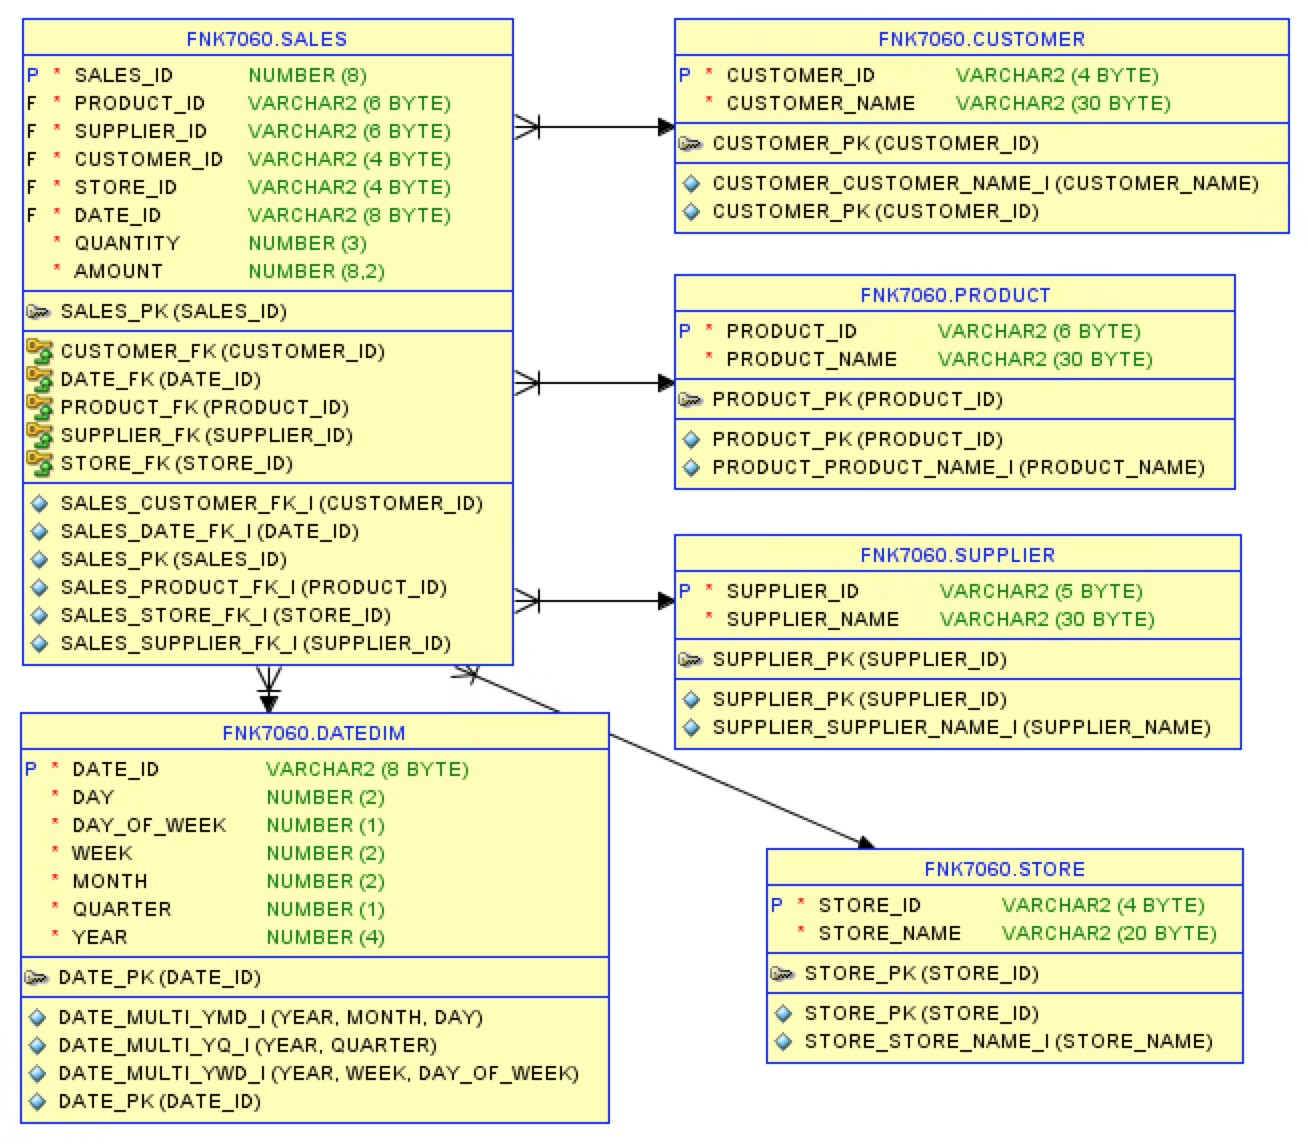
\includegraphics{./img/models.png}}
    \caption{Entity Relationship diagram generated by Oracle
    SQL Developer Data Modeler\label{fig:data-modeler}}
\end{figure}

\hypertarget{fact-table}{%
\subsection{Fact Table}\label{fact-table}}

Apparently the fact table should have foreign keys corresponding to all
five dimension tables, and the quantity of item sold. There are two
decisions have been make for primary key and amount of money in sales.
Index is created on each foreign key for performance improvement
\autocite{tripp_sqlskills_2017}.

\textbf{Primary key} of fact table can be a combination of all foreign
keys. However, there could be a concern to have more than one
transactions for the same values on all five dimensions. A quick
analysis shows that such a situation does exists, though the possibility
is low. In other words, a customer may buy one product multiple times at
one store in one day. There are two options to solve this problem. One
is summing up the quantities of multiple transactions, resulting in only
one record for the same combination of dimension values. The other is
keep multiple transactions while use a separated ID field as the primary
key of \emph{Sales} fact table. In this project, the latter solution is
preferred because this approach can keep the original granularity of
transactions, thus contains more information. Also, the possibility of
multiple transactions for one combination of dimensions is low, so there
would not be significant overhead in terms of memory and storage.

\textbf{Price/Amount} is another concerning field. In the original data,
\emph{price} is stored in master data table as a property of product, so
it is natural to make it an attribute of product dimension. However,
this design has a shortcoming when price changes as it always does. If
the price of a product changes, we cannot simply modify the value in
\emph{Product} dimension table otherwise the result on sales before that
change will be incorrect. Therefore, in this project price information
is kept in \emph{Sales} table. Since the amount of money in sales is a
more frequent used number, we add to fact table an \emph{amount} filed
which is calculated by \(\mathit{quantity}\times \mathit{price}\). In
\cref{price-attribute} further discussions will be provided on this
issue.

\hypertarget{dimensions}{%
\subsection{Dimensions}\label{dimensions}}

Details of dimension tables can be referred to \cref{fig:overall}. Most
dimensions are as simple as ``ID''+``name'', while the \emph{Date}
dimension is relatively complicated. First of all, unlike other
dimensions, there is no existing ID for \emph{Date}. In this project, a
string in format of ``YYYYMMDD'' is chosen as the ID for \emph{Date},
rather than an auto-incremental column. The advantage is such ID is more
readable and intuitive, and thus more convenient for partitioning if
required in the future \autocite{dinesh_create_nodate}. On the other
hand, it would need more storage space, which is not a big issue
providing the cost storage is quite low nowadays. Second, \emph{Date}
dimension contains more information other than names. In this project,
common properties are calculated, including \emph{year}, \emph{quarter},
\emph{month}, \emph{week}, \emph{day}, \emph{day\_of\_week}. In fact, it
can be extended to more fields such as \emph{is\_public\_holiday}, if
some analysis on holiday is in demand.

In Oracle SQL Developer, index will be created automatically on primary
key column. However, we rarely retrieve data only by primary keys
because primary key is usually an ID which is not readable to humans.
Therefore, indexes will be created on all levels of attributes in
dimension tables for fast retrieval.

\hypertarget{inlj-algorithm}{%
\section{INLJ Algorithm}\label{inlj-algorithm}}

Index Nested Loop Join (INLJ) is a table joining algorithm that can be
used for stream data joining. Nested Loop Join takes an outer loop and
an inner loop, each on one table, and output the rows that matches the
conditions, so the time complexity is \(O(N M)\) where \(N\) and \(M\)
are the number of rows of two tables. However, INLJ only keeps the outer
loop and replaces the inner loop with an index-based look-up, thus
greatly reduces the time complexity. For example, if the index is
implemented by a B-tree, then complexity of look-up is \(O(\log M)\)
instead of linear which is the case of the inner loop.

This algorithm is implemented in PL/SQL, steps shown as follows.

\begin{enumerate}
\tightlist
\item
  fetch a bulk (50 rows in this project) of transactions by cursor into
  memory.
\item
  read each row in the bulk sequentially, and for each row

  \begin{enumerate}
  \tightlist
  \item
    retrieve the information for current row from master data by
    \emph{product\_id}.
  \item
    transformed all properties into proper format
  \item
    insert values into fact and dimension tables
  \end{enumerate}
\item
  repeat step 1\textasciitilde2 until there is nothing more to fetch by
  the cursor.
\end{enumerate}

Please refer to file \emph{INLJ.sql} for the complete implementation.

\hypertarget{olap-queries-results}{%
\section{OLAP Queries Results}\label{olap-queries-results}}

This section summarises the methods and results of required analysis.
The SQL statements of these queries are referred to file
\emph{queriesDW.sql}.

\let\oldsubsection\thesubsection
\renewcommand*{\thesubsection}{Question~\arabic{subsection}}

\hypertarget{section}{%
\subsection{}\label{section}}

\begin{quote}
\textbf{Question}: Determine the top 5 products in Dec 2019 in terms of
total sales
\end{quote}

The basic idea is to calculate the sales per product in Dec 2019, then
rank the sales in descending order, and finally get first 5 ranks. The
output of query is shown as \cref{fig:q1-output}.

\begin{figure}
    \centering
    \scalebox{.7}{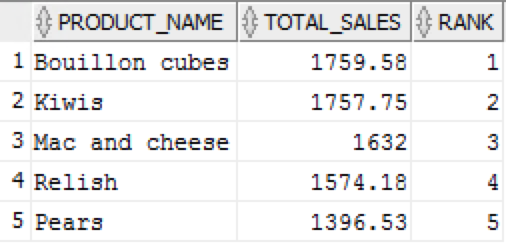
\includegraphics{./img/q1.png}}
    \caption{Query 1 Output\label{fig:q1-output}}
\end{figure}

\hypertarget{section-1}{%
\subsection{}\label{section-1}}

\begin{quote}
\textbf{Question}: Determine which store produced highest sales in the
whole year?
\end{quote}

The method is similar to previous question. The output of query is shown
as \cref{fig:q2-output}.

\begin{figure}
    \centering
    \scalebox{.7}{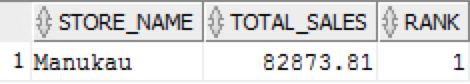
\includegraphics{./img/q2.png}}
    \caption{Query 2 Output\label{fig:q2-output}}
\end{figure}

\hypertarget{section-2}{%
\subsection{}\label{section-2}}

\begin{quote}
\textbf{Question}: Determine the top 3 products for a month (say, Dec
2019), and for the 2 months before that, in terms of total sales.
\end{quote}

The basic idea is to create a PL/SQL function that returns a collection
mimicking a table. To do this, first we need declare the types for that
collection as the return type of the function, and then use a cursor
inside the function to retrieve the data of one month. Since the cursor
is parameterised, it can be reused to query the data for any month. With
this approach we can do the analysis for any consecutive months. The
output of query is shown as \cref{fig:q3-output}.

\begin{figure}
    \centering
    \scalebox{.7}{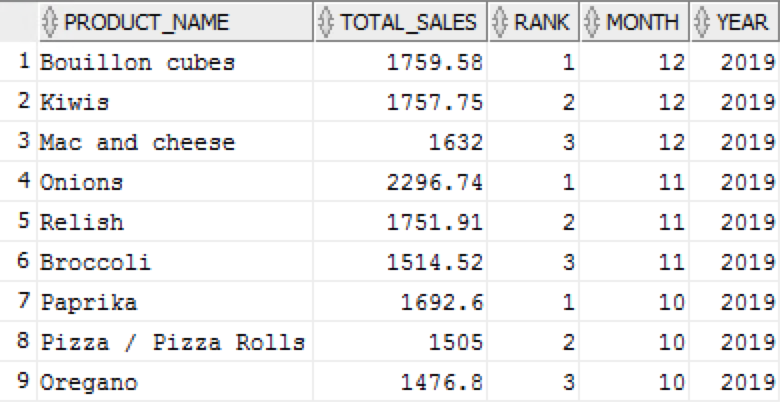
\includegraphics{./img/q3.png}}
    \caption{Query 3 Output\label{fig:q3-output}}
\end{figure}

\hypertarget{section-3}{%
\subsection{}\label{section-3}}

\begin{quote}
\textbf{Question}: Create a materialised view called ``STOREANALYSIS''
that presents the product-wise sales analysis for each store. The
results should be ordered by StoreID and then ProductID.
\end{quote}

The query is a creation statement so the output is insignificant. A
sample of rows from the materialised view is shown in
\cref{fig:q4-output}.

\begin{figure}
    \centering
    \scalebox{.7}{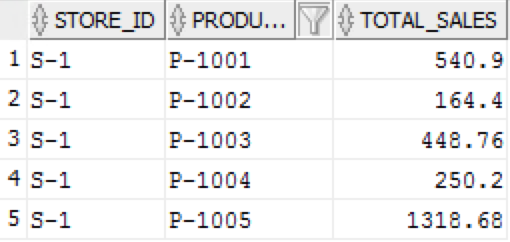
\includegraphics{./img/q4.png}}
    \caption{Query 4 Output\label{fig:q4-output}}
\end{figure}

\hypertarget{section-4}{%
\subsection{}\label{section-4}}

\begin{quote}
\textbf{Question}: Think about what information can be retrieved from
the materialised view created in Q4 using ROLLUP or CUBE concepts and
provide some useful information of your choice for management.
\end{quote}

To answer this question, a query will be created to calculate the
overall and store-wise sales, as well as the product with highest sales
in each store. \texttt{ROLLUP} is used to calculate the summation and
product-wised sales simultaneously. The output of query is shown as
\cref{fig:q5-output}.

\begin{figure}
    \centering
    \scalebox{.7}{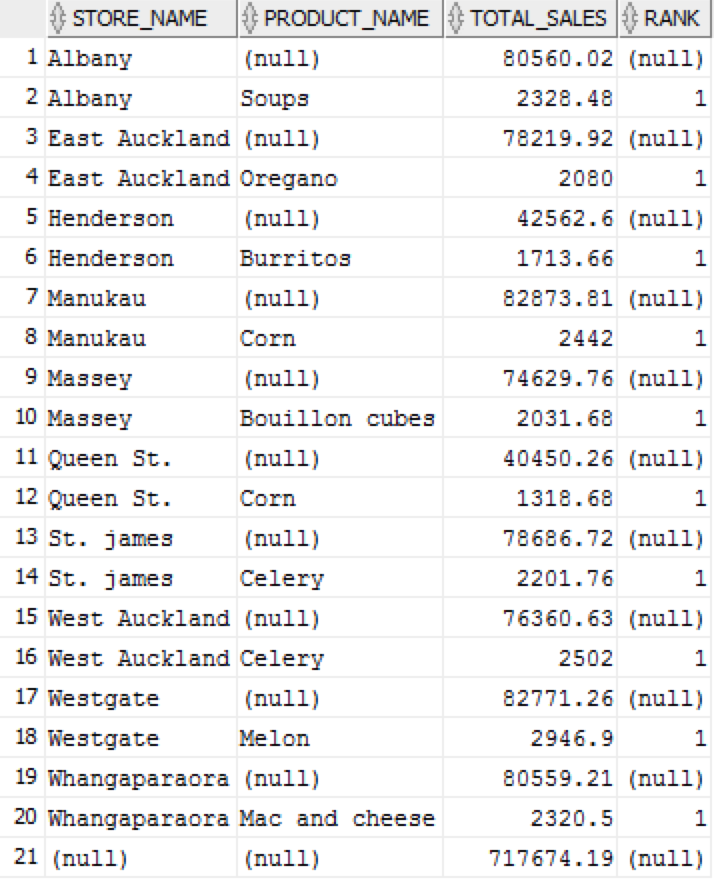
\includegraphics{./img/q5.png}}
    \caption{Query 5 Output\label{fig:q5-output}}
\end{figure}

\renewcommand*{\thesubsection}{\oldsubsection}

\hypertarget{discussion}{%
\section{Discussion}\label{discussion}}

\hypertarget{price-attribute}{%
\subsection{Price Attribute}\label{price-attribute}}

In this design, the price information is embodied in the \emph{amount}
field of fact table because of the fact that prices of products are
subject to change. However, changes of prices are way less frequent than
transactions, so there will be much redundant storage for price
information. An alternative design is to add an extra dimension
\emph{SellingItem} which is simply a combination of \emph{Product} and
\emph{price}. When price changes, a new ``selling item'' will be created
with the same \emph{product\_id} and the new \emph{price}. This method
is show in \cref{fig:alter-price}. The benefit is reducing the required
storage for price by normalisation. However, this alternative design
ends up with an architecture other than star-schema.

\begin{figure}[htbp]
  \centering
  % \sffamily
  {
  %\fontfamily{phv}\selectfont
  \fontsize{10}{11}\selectfont
  % \fontsize{7}{7}\selectfont
  %\def\svgwidth{0.9\textwidth}
    \resizebox{0.85\textwidth}{!}{\input{alternative-price-attr.pdf_tex}}
  }
  \caption{Alternative Design for Price Attribute}
  \label{fig:alter-price}
\end{figure}

\hypertarget{summary-of-learning-outcomes}{%
\section{Summary of Learning
Outcomes}\label{summary-of-learning-outcomes}}

It is a great way to learn from developing a complete DW project. The
main outcomes learned from this project includes DW design, ETL process,
DW queries, and Oracle PL/SQL and SQL features.

\hypertarget{dw-development-lifecycle}{%
\subsection{DW Development Lifecycle}\label{dw-development-lifecycle}}

The first and foremost thing I learned is how to develop a DW through
the whole lifecycle. It involves requirement analysis, schema design,
data ETL, and querying. We need to divide this complex task into
different stages, and also be able to combine them together back into a
complete and running DW project.

\hypertarget{dw-schema}{%
\subsection{DW Schema}\label{dw-schema}}

The DW is usually modelled as data cube which consists of dimensions and
measurements. In terms of physical model, dimensions are mapped to
dimension tables and measurements are mapped to fact tables. There are
two major schema for DW design, star-schema and snowflake schema. In
this project we use star-schema, which is more efficient for querying
because it has less table joints for a query. However, the disadvantage
is the lack of normalisation. Most dimensions are simple, containing
only one attributed of ``name''. However, the \emph{Date} dimension is
trickier. Decisions have been made on the choice of primary key of
\emph{date}, and what attributes should be included in this dimension.
Furthermore, constraints are applied to all fields to make all values
valid. For example, \emph{day\_of\_week} field is restricted to numbers
between 1 and 7, so an invalid value such as 8 can never been inserted
into the table.

\hypertarget{inlj-etl}{%
\subsection{INLJ \& ETL}\label{inlj-etl}}

INLJ is suitable for joining stream data with batch data in near
real-time. The key idea of INLJ of two tables is looping on the first
table and looking up on the second table through an index. Apparently,
index cannot be build on the stream data, so we can only create index on
the batch data table and loop on the stream data. It is an effective way
to avoid exhaustive search on the batch data table.

To implement INLJ in PL/SQL, ``cursor'' is an important tool. A cursor
fetches data from the output of a query, and can be traversed by a
for-loop. Cursors can fetch data row by row or in bulk. The difference
between the two manner is performance. Each time when a cursor fetches
data, there will be context switching between PL/SQL engine and SQL
engine, which incurs overhead decreasing the overall performance.
Therefore, fetching the data bulk by bulk (e.g.~50 rows at one time) can
significantly increase the execution performance. To access the data
from a cursor we need to declare variables to hold that data. We can
either declare a single variable in type of the whole row or multiple
variables each one for a specific field.

Before inserting values into dimension tables, it is necessary to check
whether that value already exists in the table or not. There are
multiple ways to check the existance of one row before insertion. In
this project a \texttt{WHERE\ NOT\ EXISTS} clause is used along with
\texttt{INSERT\ INTO\ ...\ SELECT\ ...} statement for this purpose, but
the trick here is the use of a dummy table \texttt{dual}. The reason is
as follows. The \texttt{INSERT\ INTO\ ...\ SELECT} statement will select
rows from a table and insert into the target table, but here the data to
insert actually comes from PL/SQL variables. Therefore, the dummy table
\texttt{dual} is put in the \texttt{FROM} clause, but the columns in
\texttt{SELECT} clause are actually the variables. With this approach we
can make use of \texttt{INSERT\ INTO\ ...\ SELECT} statement to check
the existence of a row before inserting it.

\hypertarget{dw-query-analysis}{%
\subsection{DW Query \& Analysis}\label{dw-query-analysis}}

Analysis on DW should be implemented by SQL queries. It usually involves
table joining so the query would be a bit complicated even for a simple
analysis.

\textbf{Top K retrieval} is a type of common analysis, which finds the
most or least measurements with corresponding dimension values. For
example, it is useful for decision-making in business operation to know
the products with K highest or lowest sales. This can be done by either
\texttt{ORDER\ BY} or \texttt{RANK()} operations in Oracle SQL
Developer. More than that, the analytics are usually done with
roll-up/drill-down/slice/dice operations. For instance, it is common to
aggregate the data of each day to month level (roll-up), or retrieve
data of a certain month (slice) or a month range (dice). For this
purpose, the \texttt{WHERE} and \texttt{GROUP\ BY} clause are used,
sometimes with \texttt{PARTITION\ BY} operation for advanced query.

\textbf{Dynamic query} is an important way to improve flexibility and
query reuse. Dynamic query is constructed in runtime with parameters
substituted by real values assigned to them. Next time if we want to do
similar analysis, we just need to change the parameter rather than
manually editing the query statement. To implement a dynamic query is
basically to create a PL/SQL table function with the query wrapped
inside it. It's called ``table function'' because it returns collections
of objects that minic tables. However, the details are somewhat
complicated. What I learned from developing a dynamic query includes:

\begin{itemize}
\tightlist
\item
  Create types of expected table for return type declaration in function
  by \texttt{CREATE\ TYPE}.
\item
  In side the function, create a parameterised cursor for data fetching.
  The parameters are about the target month, so the query can be used to
  select data of any specified month.
\item
  Use \texttt{FOR\ LOOP} and \texttt{IF\ THEN\ ELSE} to iteractively
  fetch data from database, and convert the retrieved data into the type
  matching the function declaration.
\item
  Use \texttt{PIPELINED} and \texttt{PIPE\ ROW} together to return the
  fetched records in an convenient way. Without this approach we would
  have to create a local collection, append records to it and return it
  after all data has been retrieved, but with \texttt{PIPELINED} we can
  simply ``pipe'' out each record immediately after it is retrieved
  without the needs for local collection.
\end{itemize}

\printbibliography

\end{document}
